\begin{figure}[h!]
    \centering
    \caption{Drivers of \emph{Plan Cuadrante} on Police Effectiveness}
    \label{fig:figureA4_patrol}
    \begin{subfigure}{0.495\textwidth}
        \centering
        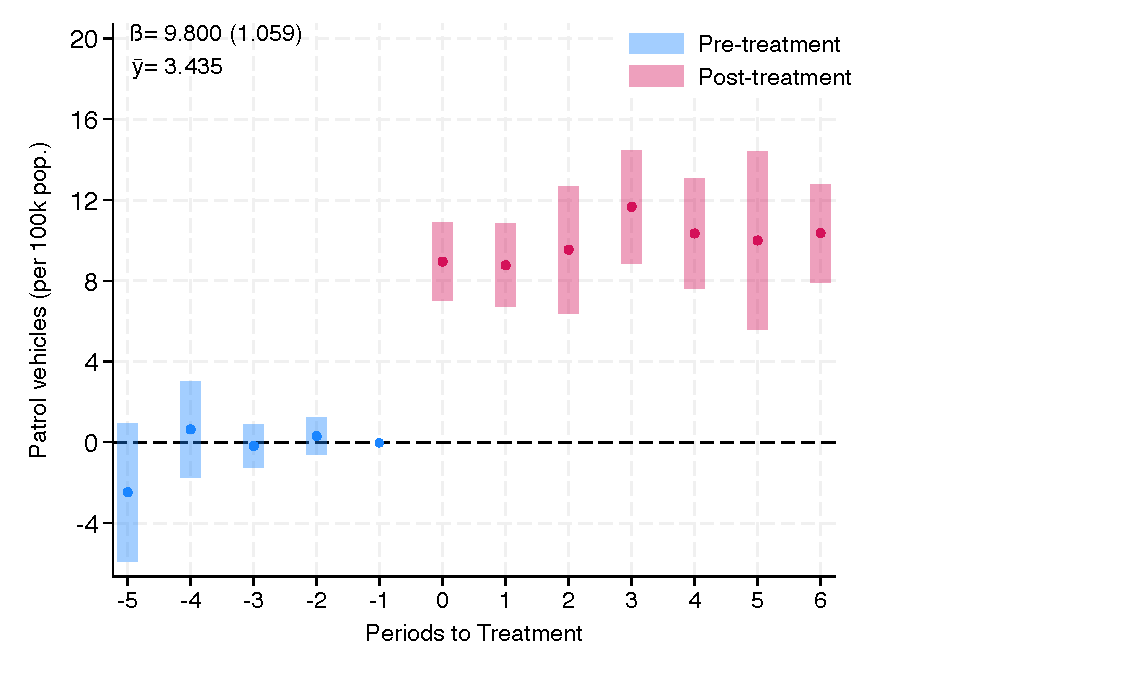
\includegraphics[width=\textwidth]{../manuscript/Graphs/results_patrols.pdf}
        \caption{$\Delta$ in Patrol Vehicles}
    \end{subfigure}%
    ~ 
    \begin{subfigure}{0.495\textwidth}
    \centering
    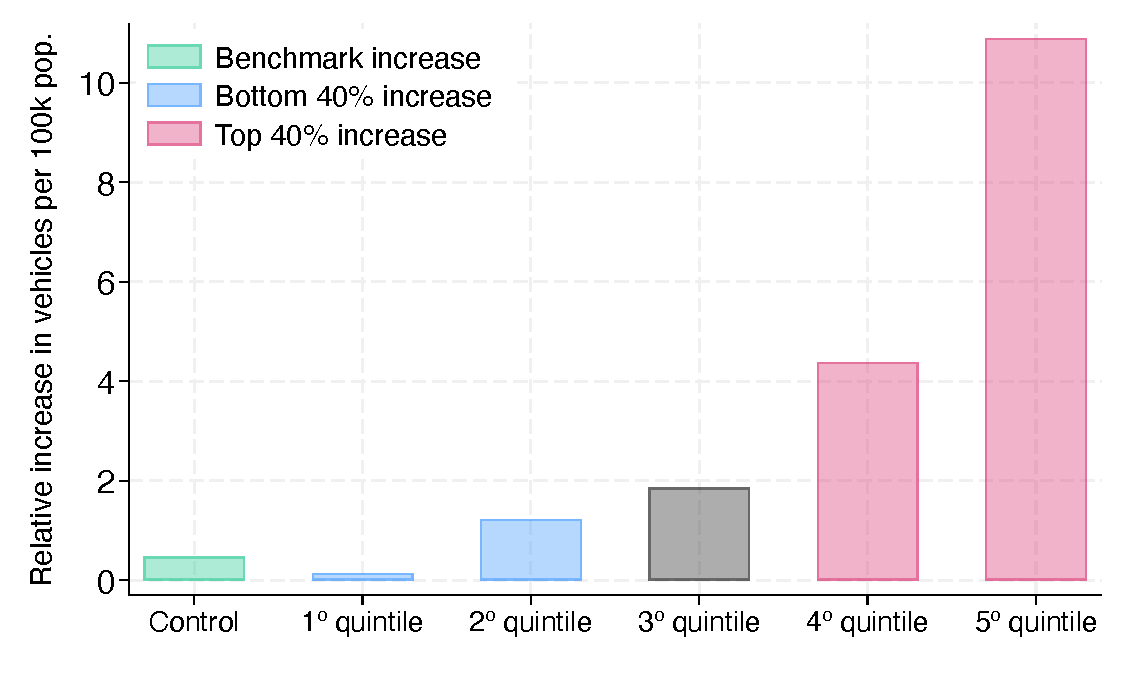
\includegraphics[width=\textwidth]{../manuscript/Graphs/mean_relintensity_patrols_quantiles.pdf}
        \caption{Distribution of $\Delta$ on Patrol Vehicles}
    \end{subfigure}
     ~ 
    \begin{subfigure}{0.495\textwidth}
    \centering
    \includegraphics[width=\textwidth]{../manuscript/Graphs/results_relintensity_patrols_quantiles.pdf}
        \caption{Effects by intensity $\Delta$ on Patrol Vehicles (ENUSC)}
    \end{subfigure}
     \begin{subfigure}{0.495\textwidth}
    \centering
    \includegraphics[width=\textwidth]{../manuscript/Graphs/results_intensity_patrols_quantiles_spd.pdf}
        \caption{Effects by intensity $\Delta$ on Patrol Vehicles (SPD)}
    \end{subfigure}
    \\[12pt]
    \begin{minipage}{0.99\textwidth}
    Notes: This figure illustrates the dynamic effects of the \emph{Plan Cuadrante} in different measures of police effectiveness. Panel (a) on the number of crimes reported to the police, panel (b) on the number of arrests. These effects were estimated using specification (\ref{eq:main}) on the sample of municipalities that adopted the \emph{Plan Cuadrante} between 2004 and 2012. For the estimation, we follow the procedure proposed by \citet{Callaway}. The dots in the figure represent the estimated coefficients and the bars behind them 95\% confidence intervals. Standard errors are clustered at the municipality level.
    \end{minipage}
\end{figure}